%************************************************
\chapter{Method validation and performance analysis on simulated data}\label{ch:simulations} 
%************************************************
\todo{Complete all the stuff that is missing. Separate the initiailization and method comparison analysis. Rewrite because this is copy paste from paper, check the references, try to fit figures in the text}
\section{Simulating data with a spatial component }
Simulating data with a spatial component is a non-trivial problem. Existing methods rely on MCMC approaches as described in \cite{Chalmond89}. However, in this case with a relatively large number of nodes in the graph ($\sim 34,000$), this is computationally expensive. To overcome this problem, I exploited the fact that the {\it{Platynereis}} dataset already possesses a spatial component. As outlined in Figure \ref{fig:simulationScheme}, the simulation starts by clustering the gene expression data using different values of $K$ with the HRMF method described in chapter \ref{ch:HMRF} and by storing the resulting parameter estimates. Subsequently, I use the values of the estimated parameter $\boldsymbol{\Theta}$ to simulate binarised gene expression data from $K$ clusters where, for cluster $h$, the expression of gene $m$ is simulated from a Bernoulli distribution with parameter $\theta_{m,h}$ as described in \ref{subsec:simul_non_spatial}. This non spatial simulated data is then reintroduced in the spatial context of the biological data \ref{subsec:simul_spatial} leading to a simulated dataset with all parameters being fully determined. In the next paragraphs, I will describe each step of this simulation scheme.

	\begin{figure}[H]
\centerline{\includegraphics[width=0.6\linewidth]{gfx/chapter5/simulation_scheme.png}}
\caption{{\bf Simulation scheme used to generate gene expression data with a spatial component and known parameters.} The values of $\Theta$ are used to generate a dataset of clusters with the same gene expression profile as the reference. Each simulated cell is then assigned to its corresponding spatial localization so that the simulated data keeps the spatial compenent of the biological data.}
\label{fig:simulationScheme}
	\end{figure}
	
	\subsection{Simulating non spatial gene expression data}\label{subsec:simul_non_spatial}
	The first step of the simulation scheme is to simulate binary gene expression data for $S=32,203$ sites and $M=86$ genes belonging to $K$ clusters. Each cluster will be assigned $N_h$ sites with $h \in [1,K]$. Given the emission model described in chapter \ref{ch:HMRF}, for each gene and each cluster, a $K \times M$ matrix $\boldsymbol{\Theta}$ is needed where each $\theta_{h,m}$ represents a Bernoulli parameter or the probability for each site in cluster $h$ to express gene $m$.\\
	
	In order to generate a biologically coherent $\boldsymbol{\Theta}$ matrix, the clustering method is applied to the biological data for $K$ clusters and the resulting final $\boldsymbol{\Theta}$ matrix is kept to simulate new data. The clustering on the biological data also gives the number of cells per cluster $N_h, \forall h \in K$.\\
	
	Once the parameters values are available it is relatively straight forward to simulate $N_h$ sites per cluster following the Bernoulli distributions thus defined resulting in $S=32,203$ sites with known $\boldsymbol{\Theta}$ parameters \todo{Appendix with R script}.
	\subsection{Introducing a known spatial context}\label{subsec:simul_spatial}
	Each simulated is then assigned to the same spatial location as the corresponding ``cube" in the biological dataset, meaning that both the simulated and the biological datasets have the same neighbouring graph. The rationale behind this simulation scheme is to allow the model to validate itself. By replacing simulated gene expression data equivalent to the biological one in the same spatial context, the hypothesis is that the set of parameters $\boldsymbol{\beta}$ will stay relatively stable when the simulated data is clustered.
	\subsection{Expected results}\label{subsec:expected_simul_results}
	Given this simulation scheme, the expected results after clustering the simulated data, is to find a strong conservation for the all the parameter $\boldsymbol{\psi} = \{\boldsymbol{\Theta},\boldsymbol{\beta}\}$ between the ``true" values $\hat{\boldsymbol{\psi}}$ obtained from clustering the biological data and the estimated values $\widetilde{\boldsymbol{\psi}}$ obtained after clustering the simulated data.

\section{Comparing clustering results using the Jaccard similarity coefficient}
	\subsection{Theoretical problem in comparing clustering results}
To compare clustering results, a lot of metrics exist to estimate the similarity between two lists of clusters. One of the widely used ones is the Jaccard coefficient \cite{jaccard1901}. For two clustering results, $A$ and $B$, the Jaccard coefficient is defined as: 
\begin{align*}
J(A,B) = \frac{|A \cap B|}{|A \cup B|}
\end{align*}
Although theoretically very simple, in practice computing this metric is not trivial. Indeed, depending on the clustering method used and on the initialization used for clustering methods that require an initialization step like the independent mixture models or the HRMF method presented in chapter \ref{ch:HMRF}, even if the clustering results are 100\% identical, they are going to be misaligned.\\

This means that for method $A$ \emph{cluster 1} could for example be \emph{cluster 5} in method $B$. In order to compute the Jaccard coefficient and compare clustering results, it is necessary to be able to align partitions. To this end I used a similarity specificity matrix approach as described in the next paragraph.


	\subsection{Alignment via similarity-specificity matric}
The ``count" matrix $D$ and the ``similarity/specificity" matrix $H$ for two sets of clusters $z$ and $z'$ with $K$ clusters each so that $z = \bigcup_{h \in [1,K]} c_h $ and $z' = \bigcup_{h \in [1,K]} c'_h$ are defined as:
\begin{align*}
D &= \left( \begin{array} {ccc}
|c_1 = c'_1| & \ldots  & |c_1 = c'_K|\\
\vdots & \ddots & \vdots\\
|c_K = c'_1| & \ldots & |c_K = c'_K| \end{array} \right)\\
\text{and}\\
H_{ij} &= \frac{D_{ij}}{\sum_{a} D_{aj} \sum_{b} D_{ib}} 
\end{align*}
With $z$ the set of reference clusters, the ones other clustering results will be aligned to (in the case of the simulation study, $z$ is the set of ``true" clusters obtained after clustering the biological data), for each row of the matrix $H$, the column with the highest value is then select as the corresponding cluster.\\

In the case of two sets of clusters being extremely similar this approach will align the cluster sets. However some errors may arise if the two cluster sets are quite different. For example if one cluster $h_{z_1}$ in $z$ is split into two clusters $h_{z'_4},h_{z'_5}$ in $z'$, they will both be assigned to $h_{z_1}$ after alignment meaning that, because $K$ is the same for $z$ and $z'$ one cluster in $z$ will have no corresponding clusters in $z'$.\\

This sort of error is central to clustering results analysis and unfortunately unavoidable. Therefore, the resulting Jaccard coefficient will not necessarily be linearly correlated with the similarity between the reference clusters and the clusters under study, instead it will have a tendency to worsen faster than the similarity due to the biases created in this alignment step. It remains however a good indication of the divergence between clustering sets. An example of aligning the clusters is shown through the values of $\boldsymbol{\Theta}$ by comparing  figures \ref{fig:theta_valid_non_aligned} and \ref{fig:theta_valid_aligned}.\\

The first thing I need to do now is to validate the correct estimation of the model's parameters. I will describe this essential step in the next section.


\section{Validation of parameters estimation and model choosing}
	\subsection{Estimation of $\boldsymbol{\Theta}$}
	To validate the consistency in estimating the values of $\boldsymbol{\Theta}$, it is important to compare the ``true" values used to simulate the data to the ones obtained after clustering the simulated data.
	A simple example with $K=6$ is presented in figure 
	
\begin{figure}[bth]
        \myfloatalign
        \subfloat[``Proximity" between values of $\boldsymbol{\Theta}$ before alignment]
        {\label{fig:theta_valid_non_aligned}
        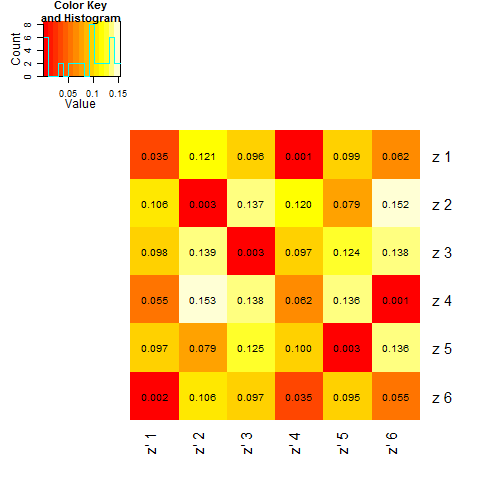
\includegraphics[width=.45\linewidth]{gfx/chapter5/heatmap6.png}} \quad
        \subfloat[``Proximity" between values of $\boldsymbol{\Theta}$ before alignment]
        {\label{fig:theta_valid_aligned}%
         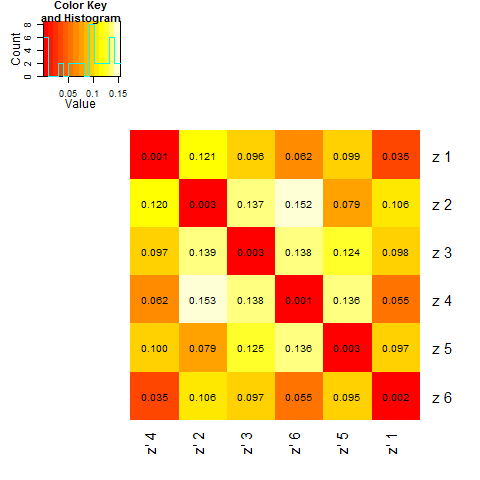
\includegraphics[width=.45\linewidth]{gfx/chapter5/heatmap6_aligned.png}}
        \caption{Validating the estimation of $\boldsymbol{\Theta}$ for $K=6$. On the x axis are shown the 6 clusters obtained after clustering the simulated data. On the y axis are shown the 6 ``true" reference clusters. Each cell of the heatmap corresponds to the mean of the pairwise (as regard to the 86 genes considered) difference between ``true" and simulated $\boldsymbol{\Theta}$ values. A small number means that the difference between the reference $\boldsymbol{\Theta}$ values and the ones obtained after clustering the simulated data is very small.}\label{fig:theta_valid}
\end{figure}
	
	The most important criterion for assessing the efficacy of our approach is the similarity between the inferred and true clusters. This also implicitly assesses the accuracy of the estimation of $\mathbf{\Theta}$: if the inferred and true clusters are identical, the estimates of $\mathbf{\Theta}$ must be equal to the true values. In practice, we used the Jaccard coefficient to compare the inferred and the true clusters (Methods), where a Jaccard coefficient of 1 implies perfect agreement. To benchmark our approach's performance, we also assessed the ability of two other models to cluster the simulated data: hierarchical clustering (hClust), a very widely used approach in genomics and elsewhere, and an independent mixture model, which allows the relative improvement in performance added by the spatial component to be studied.\\
	
		


	\subsection{Estimation of beta}\label{subsec:beta_estimation}
	As well as directly comparing the clusters, we can also determine how accurately the $\mathbf{\beta}$ parameters are estimated. To this end, in Figure \ref{fig:beta_validation} we compare the true and inferred mean values of $\mathbf{\beta}$ for different values of $K$. The values of $\mathbf{\beta}$ increase with $K$, which is to be expected since more clusters implies the existence of more transition areas, thus making an increase of $\mathbf{\beta}$ necessary to maintain the optimal spatial coherency of the model. Figure \ref{fig:beta_validation} also shows a slight but consistent underestimation of $\mathbf{\beta}$. This can be explained by noting that the simulation scheme used may reduce the spatial coherency within clusters. Specifically, as illustrated in Figure \ref{fig:beta_error}, clusters may not display homogeneous expression of a given gene: instead, depending upon the value of $\theta$, a gene will be expressed only in a fraction of cells. In reality, the cells in which such genes are expressed may have a coherent spatial structure within the cluster that is lost in the simulation, thus explaining the consistently smaller value for $\mathbf{\beta}$ that are estimated. To confirm this, we performed a second simulation using the parameter values estimated from the first simulation as a reference. In this context we did not expect any further loss of spatial coherency, which was indeed confirmed as shown by the blue curve in Figure \ref{fig:beta_validation}.\\
	
	\begin{figure}[h]
\centerline{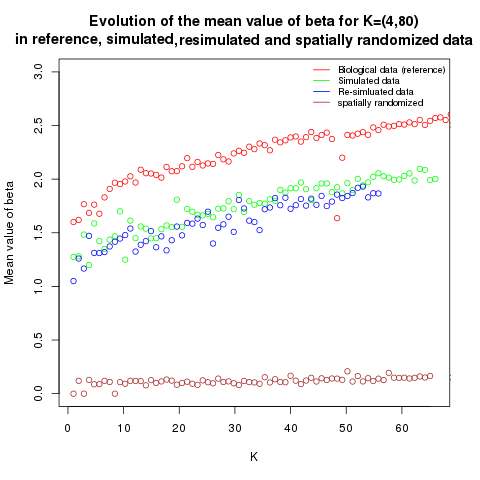
\includegraphics[width=\linewidth]{gfx/chapter5/beta_valid.png}}
\caption{{\bf Validating the estimation of beta.} This figure shows the evolution for $K \in [4,80]$ of the mean value of $\beta$ across all the clusters. The red dots represent the biological data clustering (i.e the reference in our simulations scheme). The green dots represent the results obtained after clustering simulated data, which shows an underestimation of $\beta$. To confirm that this underestimation come from the simulation scheme and not the clustering method, we used the simulated data as the reference to generate a ``second generation" of simulated data, suppressing the simulation scheme bias (see Figure \ref{fig:beta_error}). The results of this re-simulation are shown by the blue dots, which exhibit no underestimation of $\beta$. Finally the brown dots represent the mean value of $\beta$ on the same simulated data but spatially randomized, as expected the $\beta$ are now estimated to $0$.}
\label{fig:beta_validation}
	\end{figure}
	
	\begin{figure}[h]
\centerline{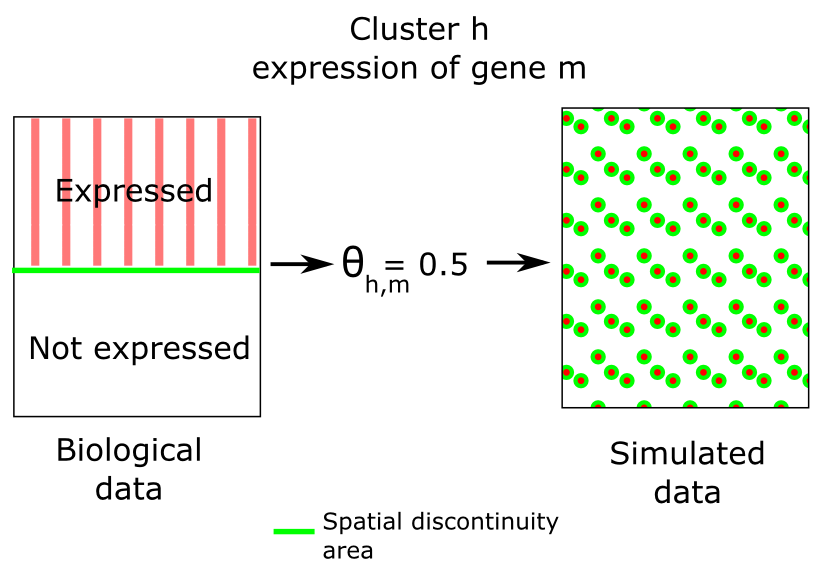
\includegraphics[width=\linewidth]{gfx/chapter5/beta_error.png}}
\caption{{\bf Decrease in spatial coherency due to the simulation scheme.} For an example cluster $h$, gene $m$ may only be expressed in half of the cells. This will yield $\theta_{h,m} = 0.5$. However, in the biological data, the cells expressing gene $m$ may be spatially coherent (i.e., located close to one another), leading to a reduced area of expression discontinuity (the green line). By contrast, in the simulated data the expression of such a gene will lose its spatial coherency, leading to an increased area of expression discontinuity. The number of cells having a neighbour with some differences in the gene expression pattern is directly linked to the value of $\beta_h$ through the energy function (Methods). This explains the underestimation of $\mathbf{\beta}$ observed in Figure \ref{fig:beta_validation}.}
\label{fig:beta_error}
	\end{figure}

To validate further our estimation of $\mathbf{\beta}$, we randomized the coordinates of the ``cubes" to lose any spatial component before re-clustering the data. As expected, we observed that the estimates of $\mathbf{\beta}$ were very close to $0$ for all clusters (Figure \ref{fig:beta_validation}),  as well as there being very similar Jaccard coefficient values (relative to the true values) for the independent mixture and the MRF model. Both of these observations provide confidence in our assertion that the spatial component plays an important role in the fit.\\



	
	The results of these experiments are shown in Figure \ref{fig:methodComparison} for $\tilde{K} \in [4,70]$. Our method, when used with a random initialization scheme (Methods), has an average Jaccard coefficient of $0.8$, and clearly demonstrates better performance than the other methods. The second best performing method is the independent mixture model with a random initialization, which has an average Jaccard coefficient of $0.7$. Since the independent mixture approach is equivalent to the MRF with all the $\beta$ parameters set equal to 0 (i.e., without a spatial component) this suggests that accounting for the spatial aspect yields improved results. Given this, it is perhaps unsurprising that hClust also performs relatively poorly. Additionally, we note that initializing the MRF with the hClust output yields results that are superior to those generated by hClust but that are still poorer than either the randomly initialized independent mixture model or the MRF approach. This is likely explained by noting that, depending upon the initialization, the EM algorithm might converge to a local maximum. Consequently, for the rest of this study we use the random initialization strategy to initialize the EM algorithm. \\
	\subsection{Choosing K}
	
Finally, we assessed the ability of the model to choose the correct number of clusters, $K$. To do this, we noted the ``true" number of clusters underlying the simulated data and compared this with the chosen value, $\hat{K}$. The results for two representative choices of $K$ are shown in Figure \ref{fig:simulatedK} and demonstrate that our clustering approach, in conjunction with the BIC, is able to accurately determine the optimal number of clusters.\\

	\begin{figure}[h]
\centerline{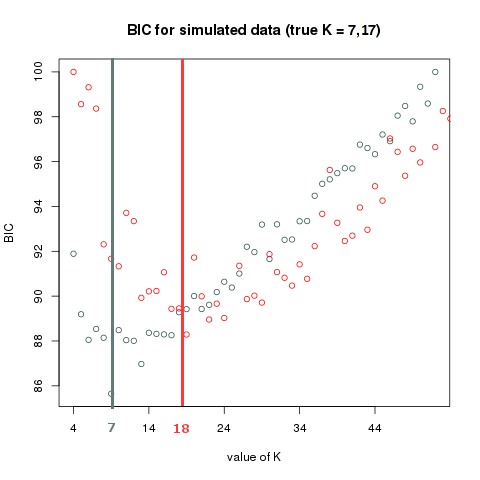
\includegraphics[width=\linewidth]{gfx/chapter5/simulated_k.png}}
\caption{{\bf Jaccard coefficient between ``true" and resulting clusters on the simulated data with different methods and initializations.} Panel A compares the performance of the MRF method with a randomly initialization with an independent mixture model also with a random initialization, the MRF method initialized with the hClust classification and hClust alone on data simulated with a spatial component. Panel B shows the Jaccard coefficient for the MRF method and independent mixture model both with a random initialization; in this case both methods are applied to simulated data that lacks a spatial component.}

\label{fig:simulatedK}
	\end{figure}

\section{Method performance and initialization}
	\subsection{Shortcomings of the EM principle}
	\subsection{Random initialization vs Hclust initialization}
	Additionally, the likelihood function that needs to be maximised possesses many stationary points of different natures. Thus, convergence to the global maximum with the Expectation-maximisation algorithm (see Methods section), depends strongly on the parameter initialisation. To overcome this problem, different initialisation strategies have been proposed and investigated (see for instance \cite{biernacki03,karlis03,mclachlan04}). Herein, we compare a random initialisation scheme with an initialisation based upon the solution obtained by applying hClust.\\

\section{Method performance compared to Hclust and independent mixture models}
	\subsection{Results of comparison}
	\begin{figure}[h]
\centerline{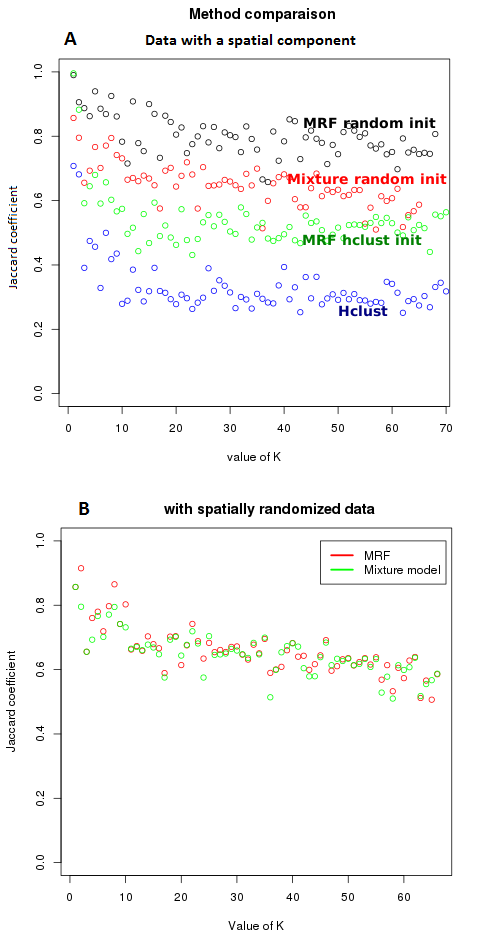
\includegraphics[width=\linewidth]{gfx/chapter5/method_comparison.png}}
\caption{{\bf Jaccard coefficient between ``true" and resulting clusters on the simulated data with different methods and initializations.} Panel A compares the performance of the MRF method with a randomly initialization with an independent mixture model also with a random initialization, the MRF method initialized with the hClust classification and hClust alone on data simulated with a spatial component. Panel B shows the Jaccard coefficient for the MRF method and independent mixture model both with a random initialization; in this case both methods are applied to simulated data that lacks a spatial component.}
\label{fig:methodComparison}
	\end{figure}
	\subsection{Discussion}





%*****************************************
%*****************************************
%*****************************************
%*****************************************
%*****************************************
